% ============================================================================
% ROBOT LOCALIZATION - EXAM NOTES
% Focus: EKF localization, feature-based maps, data association
% ============================================================================

\section{Quick Reference: EKF Localization}

\begin{tcolorbox}[colback=yellow!10!white,colframe=orange!75!black,title=\textbf{EKF Localization - Fast Reference}]

\textbf{Problem:} Estimate robot pose $x = [x, y, \theta]^T$ given:
\begin{itemize}
    \item Map $m$ with known landmark locations
    \item Motion commands $u_t = [v_t, \omega_t]^T$
    \item Sensor measurements $z_t = \{z_t^1, z_t^2, \ldots\}$ to landmarks
\end{itemize}

\vspace{3mm}
\textbf{Measurement Model (Range-Bearing):}
\begin{equation*}
z_t^i = \begin{bmatrix} r_t^i \\ \phi_t^i \\ s_t^i \end{bmatrix} = 
\begin{bmatrix} 
\sqrt{(m_{j,x} - x)^2 + (m_{j,y} - y)^2} \\ 
\arctan2(m_{j,y} - y, m_{j,x} - x) - \theta \\ 
m_{j,s} 
\end{bmatrix} + \text{noise}
\end{equation*}
where $r$ = range, $\phi$ = bearing, $s$ = signature (landmark ID feature)

\vspace{3mm}
\textbf{Measurement Jacobian $H_t$:} (Evaluated at $\bar{\mu}_t$)
\begin{equation*}
H_t^i = \begin{bmatrix} 
-\frac{\Delta x}{\sqrt{q}} & -\frac{\Delta y}{\sqrt{q}} & 0 \\[3pt]
\frac{\Delta y}{q} & -\frac{\Delta x}{q} & -1 \\[3pt]
0 & 0 & 0 
\end{bmatrix}
\end{equation*}
where $\Delta x = m_{j,x} - \bar{\mu}_{t,x}$, $\Delta y = m_{j,y} - \bar{\mu}_{t,y}$, $q = \Delta x^2 + \Delta y^2$

\vspace{3mm}
\textbf{Key Difference: Motion Model Jacobian}
\begin{itemize}
    \item $G_t$ - Jacobian of motion w.r.t. \textbf{pose} (like Lab 4)
    \item $V_t$ - Jacobian of motion w.r.t. \textbf{control} (new!)
    \item Process noise: $\bar{\Sigma}_t = G_t \Sigma_{t-1} G_t^T + V_t M_t V_t^T$
\end{itemize}

\vspace{3mm}
\textbf{Two Versions:}
\begin{enumerate}
    \item \textbf{Known correspondences:} If you know which landmark you're observing
    \item \textbf{Unknown correspondences:} Must do data association (find $\arg\max$ likelihood)
\end{enumerate}

\end{tcolorbox}

% ============================================================================
\section{The Localization Problem}
% ============================================================================

\subsection{Problem Definition}

\textbf{Localization:} Determine robot's pose $x_t = [x, y, \theta]^T$ relative to a known map $m$.

\begin{itemize}
    \item Also called \textbf{position estimation}
    \item Fundamental problem in robotics
    \item Establishes correspondence between map frame and robot's local frame
\end{itemize}

\textbf{Why is it hard?}
\begin{itemize}
    \item Pose cannot be sensed directly
    \item Single measurement usually insufficient
    \item Must integrate noisy data over time
    \item Uncertainty from both motion and sensors
\end{itemize}

\begin{figure}[H]
\centering
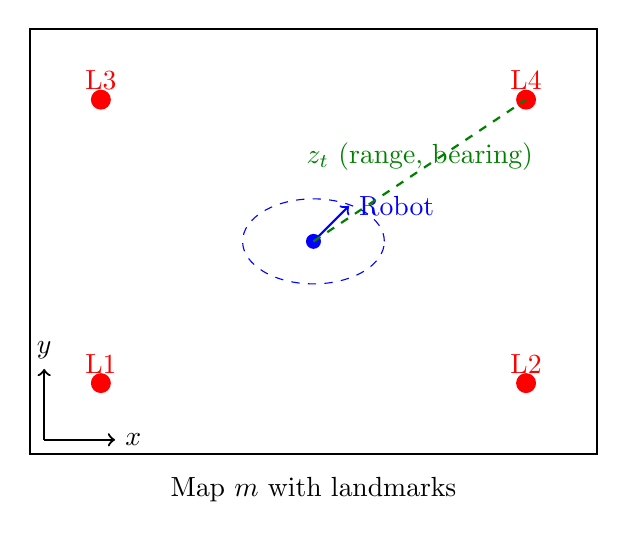
\begin{tikzpicture}[scale=0.9]
    % Draw map with landmarks
    \draw[thick] (0,0) rectangle (8,6);
    
    % Landmarks
    \foreach \x/\y/\label in {1/1/L1, 7/1/L2, 1/5/L3, 7/5/L4} {
        \fill[red] (\x,\y) circle (4pt);
        \node[red, above] at (\x,\y) {\label};
    }
    
    % Robot (with uncertainty ellipse)
    \fill[blue] (4,3) circle (3pt);
    \draw[->, thick, blue] (4,3) -- (4.5,3.5) node[right] {Robot};
    \draw[blue, dashed] (4,3) ellipse (1cm and 0.6cm);
    
    % Measurement to landmark
    \draw[green!50!black, thick, dashed] (4,3) -- (7,5);
    \node[green!50!black] at (5.5,4.2) {$z_t$ (range, bearing)};
    
    % Coordinate frame
    \draw[->, thick] (0.2,0.2) -- (1.2,0.2) node[right] {$x$};
    \draw[->, thick] (0.2,0.2) -- (0.2,1.2) node[above] {$y$};
    
    \node at (4,-0.5) {Map $m$ with landmarks};
\end{tikzpicture}
\caption{Localization: estimate robot pose given map and measurements to landmarks}
\end{figure}

\subsection{Three Types of Localization Problems}

\begin{tcolorbox}[colback=blue!5!white,colframe=blue!75!black,title=Localization Problem Types]

\textbf{1. Position Tracking}
\begin{itemize}
    \item Initial pose is \textbf{known}
    \item Track small deviations over time
    \item Initial belief: $bel(x_0) = \delta(\bar{x}_0)$ (point-mass at known pose)
    \item \textbf{Easier problem} - local, unimodal
\end{itemize}

\textbf{2. Global Localization}
\begin{itemize}
    \item Initial pose is \textbf{unknown}
    \item Must determine pose from scratch
    \item Initial belief: $bel(x_0) = \frac{1}{|X|}$ (uniform over all valid poses)
    \item \textbf{Harder problem} - global, potentially multi-modal
\end{itemize}

\textbf{3. Kidnapped Robot Problem}
\begin{itemize}
    \item Robot is "kidnapped" and moved to unknown location during operation
    \item Must detect that localization has failed and re-localize
    \item \textbf{Hardest problem} - requires fault detection
\end{itemize}

\end{tcolorbox}

\textbf{Note:} EKF localization (Gaussian) is best for position tracking. Global localization often requires multi-hypothesis methods (particle filters, grid-based methods).

% ============================================================================
\section{Markov Localization (General Framework)}
% ============================================================================

\textbf{Markov localization} is the direct application of Bayes filter to localization.

\subsection{The Algorithm}

\begin{algorithm}[H]
\caption{Markov Localization}
\KwInput{$bel(x_{t-1})$, $u_t$, $z_t$, map $m$}
\KwOutput{$bel(x_t)$}

\BlankLine
\tcp{Prediction Step}
\For{all $x_t$}{
    $\bar{bel}(x_t) = \int p(x_t \mid u_t, x_{t-1}, m) \cdot bel(x_{t-1}) \, dx_{t-1}$\;
}

\BlankLine
\tcp{Correction Step}
\For{all $x_t$}{
    $bel(x_t) = \eta \cdot p(z_t \mid x_t, m) \cdot \bar{bel}(x_t)$\;
}

\BlankLine
\Return{$bel(x_t)$}
\end{algorithm}

\textbf{Key differences from basic Bayes filter:}
\begin{itemize}
    \item Map $m$ is given and fixed
    \item Motion model: $p(x_t \mid u_t, x_{t-1}, m)$ - may use map (e.g., for collision detection)
    \item Measurement model: $p(z_t \mid x_t, m)$ - compares observation to expected measurement from map
\end{itemize}

% ============================================================================
\section{EKF Localization: Feature-Based Maps}
% ============================================================================

\subsection{Map Representation}

\textbf{Feature-based map:} Collection of point landmarks
\begin{equation}
m = \{m_1, m_2, \ldots, m_N\}
\end{equation}

Each landmark $m_j$ has:
\begin{equation}
m_j = [m_{j,x}, m_{j,y}, m_{j,s}]^T
\end{equation}
where:
\begin{itemize}
    \item $(m_{j,x}, m_{j,y})$ - landmark location in global frame
    \item $m_{j,s}$ - landmark signature (unique identifier or feature descriptor)
\end{itemize}

\subsection{Measurement Model}

At time $t$, robot observes multiple features: $z_t = \{z_t^1, z_t^2, \ldots, z_t^{k_t}\}$

Each measurement $z_t^i$ consists of:
\begin{equation}
z_t^i = \begin{bmatrix} r_t^i \\ \phi_t^i \\ s_t^i \end{bmatrix}
\end{equation}

\begin{itemize}
    \item $r_t^i$ - \textbf{range} (distance) to landmark
    \item $\phi_t^i$ - \textbf{bearing} (angle) to landmark relative to robot heading
    \item $s_t^i$ - \textbf{signature} of landmark (what type/ID it is)
\end{itemize}

\begin{figure}[H]
\centering
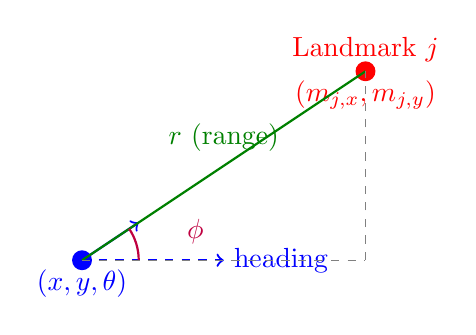
\begin{tikzpicture}[scale=1.2]
    % Robot
    \fill[blue] (2,2) circle (3pt);
    \draw[->, thick, blue] (2,2) -- (2.6,2.4);
    \node[blue, below] at (2,2) {$(x, y, \theta)$};
    
    % Robot heading
    \draw[->, thick, blue, dashed] (2,2) -- (3.5,2) node[right] {heading};
    
    % Landmark
    \fill[red] (5,4) circle (3pt);
    \node[red, above] at (5,4) {Landmark $j$};
    \node[red, below] at (5,4) {$(m_{j,x}, m_{j,y})$};
    
    % Range
    \draw[green!50!black, thick] (2,2) -- (5,4);
    \node[green!50!black] at (3.5,3.3) {$r$ (range)};
    
    % Bearing angle
    \draw[purple, thick] (2.6,2) arc (0:33.7:0.6);
    \node[purple] at (3.2,2.3) {$\phi$};
    
    % Angle measurement
    \draw[gray, dashed] (2,2) -- (5,2);
    \draw[gray, dashed] (5,2) -- (5,4);
\end{tikzpicture}
\caption{Range-bearing measurement model}
\end{figure}

\subsection{Expected Measurement Function}

Given robot pose $x = [x, y, \theta]^T$ and landmark $m_j$, expected measurement is:

\begin{equation}
\boxed{
h(x, m_j) = \begin{bmatrix} 
\sqrt{(m_{j,x} - x)^2 + (m_{j,y} - y)^2} \\[5pt]
\arctan2(m_{j,y} - y, m_{j,x} - x) - \theta \\[5pt]
m_{j,s} 
\end{bmatrix}
}
\label{eq:measurement_function}
\end{equation}

Let $\Delta x = m_{j,x} - x$, $\Delta y = m_{j,y} - y$, and $q = \Delta x^2 + \Delta y^2$. Then:

\begin{equation}
h(x, m_j) = \begin{bmatrix} \sqrt{q} \\ \arctan2(\Delta y, \Delta x) - \theta \\ m_{j,s} \end{bmatrix}
\end{equation}

\textbf{Actual measurement:} $z_t^i = h(x_t, m_j) + \epsilon$ where $\epsilon \sim \mathcal{N}(0, Q_t)$

\subsection{Measurement Jacobian}

To linearize for EKF, compute Jacobian w.r.t. robot pose:

\begin{equation}
H_t^i = \frac{\partial h}{\partial x}\bigg|_{x=\bar{\mu}_t} = 
\boxed{
\begin{bmatrix} 
-\frac{\Delta x}{\sqrt{q}} & -\frac{\Delta y}{\sqrt{q}} & 0 \\[5pt]
\frac{\Delta y}{q} & -\frac{\Delta x}{q} & -1 \\[5pt]
0 & 0 & 0 
\end{bmatrix}
}
\label{eq:measurement_jacobian}
\end{equation}

where all quantities evaluated at predicted pose $\bar{\mu}_t$:
\begin{align}
\Delta x &= m_{j,x} - \bar{\mu}_{t,x} \\
\Delta y &= m_{j,y} - \bar{\mu}_{t,y} \\
q &= \Delta x^2 + \Delta y^2
\end{align}

\textbf{Derivation notes:}
\begin{itemize}
    \item Row 1: $\frac{\partial}{\partial x}[\sqrt{q}] = \frac{1}{2\sqrt{q}} \cdot 2\Delta x \cdot (-1) = -\frac{\Delta x}{\sqrt{q}}$
    \item Row 2: $\frac{\partial}{\partial x}[\arctan2(\Delta y, \Delta x)] = \frac{\Delta y}{q}$ (chain rule on atan)
    \item Row 3: Signature doesn't depend on robot pose
\end{itemize}

\begin{tcolorbox}[colback=green!5!white,colframe=green!60!black,title=Understanding the Jacobian]

\textbf{Physical interpretation of $H_t$:}

\begin{itemize}
    \item \textbf{Row 1:} How range $r$ changes with small pose changes
    \begin{itemize}
        \item Moving toward landmark ($+\Delta x$ if landmark is to the right) decreases range
        \item Hence negative sign
    \end{itemize}
    
    \item \textbf{Row 2:} How bearing $\phi$ changes with small pose changes
    \begin{itemize}
        \item Moving perpendicular to line-of-sight changes bearing most
        \item Robot rotation directly affects bearing (hence $-1$ in $\theta$ column)
    \end{itemize}
    
    \item \textbf{Row 3:} Signature independent of pose (all zeros)
\end{itemize}

\end{tcolorbox}

% ============================================================================
\section{Motion Model for Localization}
% ============================================================================

EKF localization typically uses the \textbf{velocity motion model}:

\begin{equation}
x_t = x_{t-1} + \begin{bmatrix}
-\frac{v_t}{\omega_t}\sin\theta + \frac{v_t}{\omega_t}\sin(\theta + \omega_t\Delta t) \\
\frac{v_t}{\omega_t}\cos\theta - \frac{v_t}{\omega_t}\cos(\theta + \omega_t\Delta t) \\
\omega_t\Delta t
\end{bmatrix} + \epsilon
\end{equation}

\subsection{Two Jacobians for Motion Model}

\textbf{1. Jacobian w.r.t. state $G_t$:} (Like Lab 4)
\begin{equation}
G_t = \frac{\partial g}{\partial x}\bigg|_{x=\mu_{t-1}} = 
\begin{bmatrix} 
1 & 0 & -\frac{v_t}{\omega_t}\cos\theta + \frac{v_t}{\omega_t}\cos(\theta + \omega_t\Delta t) \\
0 & 1 & -\frac{v_t}{\omega_t}\sin\theta + \frac{v_t}{\omega_t}\sin(\theta + \omega_t\Delta t) \\
0 & 0 & 1 
\end{bmatrix}
\end{equation}

\textbf{2. Jacobian w.r.t. control $V_t$:} (New for localization!)
\begin{equation}
V_t = \frac{\partial g}{\partial u}\bigg|_{u=u_t} = 
\begin{bmatrix}
\frac{-\sin\theta + \sin(\theta+\omega_t\Delta t)}{\omega_t} & \frac{v_t(\sin\theta - \sin(\theta+\omega_t\Delta t))}{\omega_t^2} + \frac{v_t\cos(\theta+\omega_t\Delta t)\Delta t}{\omega_t} \\
\frac{\cos\theta - \cos(\theta+\omega_t\Delta t)}{\omega_t} & -\frac{v_t(\cos\theta - \cos(\theta+\omega_t\Delta t))}{\omega_t^2} + \frac{v_t\sin(\theta+\omega_t\Delta t)\Delta t}{\omega_t} \\
0 & \Delta t
\end{bmatrix}
\end{equation}

\textbf{Control noise covariance:}
\begin{equation}
M_t = \begin{bmatrix} 
\alpha_1 v_t^2 + \alpha_2 \omega_t^2 & 0 \\ 
0 & \alpha_3 v_t^2 + \alpha_4 \omega_t^2 
\end{bmatrix}
\end{equation}

\textbf{Predicted covariance:}
\begin{equation}
\boxed{\bar{\Sigma}_t = G_t \Sigma_{t-1} G_t^T + V_t M_t V_t^T}
\end{equation}

This accounts for:
\begin{itemize}
    \item Uncertainty propagation from previous pose ($G_t \Sigma_{t-1} G_t^T$)
    \item Control noise ($V_t M_t V_t^T$)
\end{itemize}

% ============================================================================
\section{EKF Localization Algorithm}
% ============================================================================

\subsection{Version 1: Known Correspondences}

\textbf{Assumption:} For each measurement $z_t^i$, we know which landmark $c_t^i = j$ it corresponds to.

\begin{algorithm}[H]
\caption{EKF Localization (Known Correspondences)}
\KwInput{$\mu_{t-1}$, $\Sigma_{t-1}$, $u_t$, $z_t$, $c_t$, map $m$}
\KwOutput{$\mu_t$, $\Sigma_t$}

\BlankLine
\tcp{PREDICTION STEP}
Compute $G_t$, $V_t$, $M_t$ from motion model\;
$\bar{\mu}_t = \mu_{t-1} + g(u_t, \mu_{t-1})$ \tcp{predicted mean}
$\bar{\Sigma}_t = G_t \Sigma_{t-1} G_t^T + V_t M_t V_t^T$ \tcp{predicted covariance}

\BlankLine
\tcp{CORRECTION STEP (for each observed feature)}
$Q_t = \text{diag}(\sigma_r^2, \sigma_\phi^2, \sigma_s^2)$ \tcp{measurement noise}

\For{each observed feature $z_t^i = [r_t^i, \phi_t^i, s_t^i]^T$}{
    $j = c_t^i$ \tcp{known correspondence}
    
    \tcp{Compute expected measurement}
    $\Delta x = m_{j,x} - \bar{\mu}_{t,x}$, $\Delta y = m_{j,y} - \bar{\mu}_{t,y}$, $q = \Delta x^2 + \Delta y^2$\;
    $\hat{z}_t^i = \begin{bmatrix} \sqrt{q} \\ \arctan2(\Delta y, \Delta x) - \bar{\mu}_{t,\theta} \\ m_{j,s} \end{bmatrix}$\;
    
    \tcp{Compute measurement Jacobian}
    $H_t^i = \begin{bmatrix} 
    -\frac{\Delta x}{\sqrt{q}} & -\frac{\Delta y}{\sqrt{q}} & 0 \\
    \frac{\Delta y}{q} & -\frac{\Delta x}{q} & -1 \\
    0 & 0 & 0 
    \end{bmatrix}$\;
    
    \tcp{Kalman gain and update}
    $S_t^i = H_t^i \bar{\Sigma}_t [H_t^i]^T + Q_t$ \tcp{innovation covariance}
    $K_t^i = \bar{\Sigma}_t [H_t^i]^T [S_t^i]^{-1}$ \tcp{Kalman gain}
    $\bar{\mu}_t = \bar{\mu}_t + K_t^i (z_t^i - \hat{z}_t^i)$ \tcp{update mean}
    $\bar{\Sigma}_t = (I - K_t^i H_t^i) \bar{\Sigma}_t$ \tcp{update covariance}
}

\BlankLine
$\mu_t = \bar{\mu}_t$, $\Sigma_t = \bar{\Sigma}_t$\;
\Return{$\mu_t$, $\Sigma_t$}
\end{algorithm}

\textbf{Key points:}
\begin{itemize}
    \item Process measurements \textbf{sequentially}
    \item Each measurement refines the belief
    \item After all measurements: $\mu_t$ and $\Sigma_t$ are final estimates
\end{itemize}

% ============================================================================
\subsection{Version 2: Unknown Correspondences (Data Association)}
% ============================================================================

\textbf{Problem:} We don't know which landmark each measurement corresponds to!

\textbf{Solution:} For each measurement, find the landmark that best explains it (maximum likelihood).

\begin{tcolorbox}[colback=red!5!white,colframe=red!75!black,title=The Data Association Problem]

Given measurement $z_t^i$, which landmark $j$ in the map did it come from?

\textbf{Approach:} Test all landmarks, pick most likely:
\begin{equation}
j^*(i) = \arg\max_j \, p(z_t^i \mid \bar{\mu}_t, m_j)
\end{equation}

This is a \textbf{maximum likelihood} correspondence estimator.

\textbf{The likelihood:}
\begin{equation}
p(z_t^i \mid \bar{\mu}_t, m_j) = \det(2\pi S_t^j)^{-1/2} \exp\left\{-\frac{1}{2}(z_t^i - \hat{z}_t^j)^T [S_t^j]^{-1} (z_t^i - \hat{z}_t^j)\right\}
\end{equation}

where $\hat{z}_t^j$ is expected measurement from landmark $j$ and $S_t^j$ is innovation covariance.

\end{tcolorbox}

\begin{algorithm}[H]
\caption{EKF Localization (Unknown Correspondences)}
\KwInput{$\mu_{t-1}$, $\Sigma_{t-1}$, $u_t$, $z_t$, map $m$}
\KwOutput{$\mu_t$, $\Sigma_t$}

\BlankLine
\tcp{PREDICTION STEP (same as before)}
Compute $G_t$, $V_t$, $M_t$\;
$\bar{\mu}_t = \mu_{t-1} + g(u_t, \mu_{t-1})$\;
$\bar{\Sigma}_t = G_t \Sigma_{t-1} G_t^T + V_t M_t V_t^T$\;

\BlankLine
\tcp{CORRECTION WITH DATA ASSOCIATION}
$Q_t = \text{diag}(\sigma_r^2, \sigma_\phi^2, \sigma_s^2)$\;

\For{each observed feature $z_t^i$}{
    \tcp{Test all landmarks to find best match}
    \For{each landmark $k$ in map $m$}{
        Compute $\hat{z}_t^k$, $H_t^k$, $S_t^k$ as before\;
        Compute likelihood $\mathcal{L}_k = \det(2\pi S_t^k)^{-1/2} \exp\{-\frac{1}{2}(z_t^i - \hat{z}_t^k)^T [S_t^k]^{-1} (z_t^i - \hat{z}_t^k)\}$\;
    }
    
    \tcp{Pick landmark with maximum likelihood}
    $j^*(i) = \arg\max_k \mathcal{L}_k$\;
    
    \tcp{Update with best correspondence}
    $K_t^i = \bar{\Sigma}_t [H_t^{j^*}]^T [S_t^{j^*}]^{-1}$\;
    $\bar{\mu}_t = \bar{\mu}_t + K_t^i (z_t^i - \hat{z}_t^{j^*})$\;
    $\bar{\Sigma}_t = (I - K_t^i H_t^{j^*}) \bar{\Sigma}_t$\;
}

\BlankLine
$\mu_t = \bar{\mu}_t$, $\Sigma_t = \bar{\Sigma}_t$\;
\Return{$\mu_t$, $\Sigma_t$}
\end{algorithm}

\textbf{Computational complexity:}
\begin{itemize}
    \item $k_t$ measurements, $N$ landmarks
    \item Must compute $k_t \times N$ likelihoods
    \item Can be slow for large maps!
\end{itemize}

% ============================================================================
\section{Practical Considerations}
% ============================================================================

\subsection{Data Association Challenges}

\begin{tcolorbox}[colback=red!5!white,colframe=red!75!black,title=When Data Association Fails]

\textbf{Perceptual aliasing:} Multiple landmarks look similar
\begin{itemize}
    \item Trees in a forest all look alike
    \item Corners in a building all look alike
    \item Maximum likelihood may pick wrong landmark!
\end{itemize}

\textbf{Consequences of wrong association:}
\begin{itemize}
    \item Innovation $(z_t^i - \hat{z}_t^{j^*})$ is large
    \item Update pulls pose estimate in wrong direction
    \item Can cause \textbf{filter divergence}
\end{itemize}

\textbf{Mitigation strategies:}
\begin{enumerate}
    \item Use distinctive landmarks (good signatures $s$)
    \item Multi-hypothesis tracking (keep multiple hypotheses)
    \item Validation gates (reject measurements with very low likelihood)
    \item RANSAC or other robust estimation
\end{enumerate}

\end{tcolorbox}

\subsection{Computational Efficiency}

\begin{itemize}
    \item \textbf{Efficient search:} Don't test all landmarks
    \begin{itemize}
        \item Project measurement into world frame
        \item Only test nearby landmarks
        \item Spatial data structures (kd-tree, octree)
    \end{itemize}
    
    \item \textbf{Batch processing:} Can process multiple measurements together (matrix operations)
    
    \item \textbf{Sparse updates:} Not all landmarks visible at once
\end{itemize}

\subsection{Limitations of EKF Localization}

\begin{enumerate}
    \item \textbf{Unimodal:} Cannot handle global localization well
    \begin{itemize}
        \item Gaussian assumption = single hypothesis
        \item If initial pose very uncertain, may converge to wrong location
    \end{itemize}
    
    \item \textbf{Linearization errors:} Large uncertainties or high nonlinearity can cause issues
    
    \item \textbf{Data association:} Hard decision - once made, can't be undone
    
    \item \textbf{Map required:} Must have map with known landmarks
\end{enumerate}

\textbf{When EKF localization works well:}
\begin{itemize}
    \item Initial pose approximately known (position tracking)
    \item Distinctive landmarks
    \item Low to moderate nonlinearity
    \item Reasonably accurate sensors and motion
\end{itemize}

% ============================================================================
\section{Comparison: Localization vs. SLAM}
% ============================================================================

\begin{tcolorbox}[colback=green!5!white,colframe=green!60!black]

\textbf{EKF Localization:}
\begin{itemize}
    \item \textbf{Given:} Map $m$ (landmark locations known)
    \item \textbf{Estimate:} Robot pose $x_t$ only
    \item State dimension: 3 (just robot pose)
\end{itemize}

\textbf{EKF SLAM (Simultaneous Localization and Mapping):}
\begin{itemize}
    \item \textbf{Given:} Nothing (no map)
    \item \textbf{Estimate:} Robot pose $x_t$ AND landmark locations $m$
    \item State dimension: $3 + 2N$ (robot + $N$ 2D landmarks)
    \item Much more complex!
\end{itemize}

\end{tcolorbox}

% ============================================================================
\section{Exam Preparation Summary}
% ============================================================================

\begin{tcolorbox}[colback=red!10!white,colframe=red!75!black,title=\textbf{Key Concepts for Exam}]

\textbf{1. Understand the problem:}
\begin{itemize}
    \item Localization = estimate robot pose given map
    \item Three types: tracking, global, kidnapped robot
    \item EKF best for tracking (unimodal)
\end{itemize}

\textbf{2. Measurement model:}
\begin{itemize}
    \item Range-bearing: $z = [r, \phi, s]^T$
    \item Formula: $h(x, m_j)$ (memorize or derive quickly)
    \item Jacobian $H_t$ structure and meaning
\end{itemize}

\textbf{3. Data association:}
\begin{itemize}
    \item Known correspondences: straightforward
    \item Unknown correspondences: max likelihood over all landmarks
    \item Key challenge in real systems
\end{itemize}

\textbf{4. Algorithm structure:}
\begin{itemize}
    \item Predict: motion model (like Lab 4, but with $V_t M_t V_t^T$)
    \item Update: sequential for each measurement
    \item Each measurement refines belief
\end{itemize}

\textbf{5. Practical issues:}
\begin{itemize}
    \item Wrong correspondences cause divergence
    \item Computational cost: $O(k_t \times N)$ per timestep
    \item Linearization limits (small uncertainty needed)
\end{itemize}

\end{tcolorbox}

% ============================================================================
% END OF LOCALIZATION NOTES
% ============================================================================
